\documentclass[a4,10pt]{article}
\usepackage[includeheadfoot,left=2cm,right=2cm,top=2cm,bottom=2cm]{geometry}
\usepackage{titling}
\usepackage{graphicx}

\usepackage[dvipsnames]{xcolor}

\usepackage{hyperref}
\hypersetup{colorlinks=true, linktocpage=true, pdfstartpage=1, pdfstartview=FitV,%
	breaklinks=true, pdfpagemode=UseNone, pageanchor=true, pdfpagemode=UseOutlines,%
	plainpages=false, bookmarksnumbered, bookmarksopen=true, bookmarksopenlevel=1,%
	hypertexnames=true, pdfhighlight=/O,
	urlcolor=RoyalBlue, linkcolor=RoyalBlue, citecolor=RoyalBlue,
	pdftitle={Multivariate Geochemical Tectonic Discrimination: Practical Approaches, Limitations and Opportunities},%
	pdfauthor={\textcopyright Morgan Williams}}

\makeatletter
\newcommand\fref[2]{\hyper@linkurl{#2}{#1}}
\makeatother

\usepackage[round, authoryear]{natbib}
\usepackage{multicol}
\usepackage{setspace}
\setlength{\columnsep}{0.6cm}
\bibliographystyle{bibstyle} 
\newcommand*{\doi}[1]{\href{https://doi.org/\detokenize{#1}}{doi: \detokenize{#1}}}
\renewcommand{\bibsection}{}%\renewcommand\bibsection{\chapter{\bibname}}%
\renewcommand{\bibname}{References}

\date{}
\title{Multivariate Geochemical Tectonic Discrimination:\\Practical Approaches, Limitations and Opportunities}
\author{Morgan Williams, Jens Klump \& Steve Barnes\\\footnotesize{\textit{CSIRO Mineral Resources, ARRC, Kensington, WA}}}

\begin{document}
		
	\maketitle

	\subsection*{Summary}
	
	Modern machine learning approaches to multivariate geochemical tectonic discrimination overcome limitations of classical graphical methods and leverage large public geochemical databases to achieve high classification accuracy. Here we document practical approaches to developing classification models using free and open source tools and investigate methods for visualising classification uncertainties and high-dimensional spatial relationships. In applying these classification methods into deep time, issues of biases and secular change become apparent. We discuss some opportunities to build upon these models and provide richer insight for future classification models.
	
	\begin{multicols*}{2}[]
	
	\subsection*{Introduction}
	
	Whole rock geochemistry is widely used to constrain the tectonic context in which magmatic rocks have been formed, with varying levels of success. Tectonic discrimination using whole-rock geochemical data is complicated by long geological histories, alteration, biased preservation and secular change. The most prevalent tectonic discrimination methods involve relatively few geochemical parameters, being historically limited by the ability to create graphical representations \citep[i.e. bivariate or ternary discrimination diagrams;][]{Pearce1973}. Many of these use geochemical proxies to encode information about geological processes or \citep[e.g. the "Pearce diagrams" which use Th/Yb, Nb/Yb and TiO\textsubscript{2}/Yb as proxies for subduction influence, source enrichment and depth of mantle melting respectively;][]{Pearce2008}, while others are designed to provide optimal discrimination for a specific scenario. While a wide variety of geochemical proxies can be used with relative confidence to discriminate between modern rocks, investigating primary geochemical contrast in ancient rocks (especially into the Archean) requires restriction of variables considered to those which are least effected by geological modification, i.e. immobile elements such as the High Field Strength Elements (HFSE) and Rare Earth Elements (REE). The limited perspective of some of these methods can lead to variable and uncertain classifications depending on the elements chosen, especially when applied into deep time. 
	
	Recent studies centred on the use of machine tectonic discrimination of magmatic rocks expand tectonic discrimination models to higher dimensions to achieve improved resolution of geochemical contrast \citep[using support vector machines, random forests and sparse multinomial regression;][]{Petrelli2016,Ueki2018}. These investigations reveal that tectonic discrimination of modern rocks can be conducted with up to approximately 90\% accuracy, if sufficient geochemical components are included (17-29, including major and trace elements, and isotopes).
	
	These recently explored methods are enabled by the development of large public geochemical and petrological databases such as EarthChem \citep[][]{Lehnert2000} and GEOROC, which  together contain millions of individual geochemical analyses, and provide an asset which is currently underutilised. The breadth and variety coupled with the volume of these databases allow the repositories to be practically useful for both high-level and specific geochemical studies, and especially classification tasks. This data requires varying levels of formatting, aggregation and transformation, particularly when integrating multiple data sources. We have developed an open-source python package focused on geochemical data processing, transformation and visualisation  \citep[][]{Williams2019}. This package includes methods for working with compositional data, aggregation and recalculation of geochemical variables, and a variety of plotting tasks. It includes components for using geochemical data in constructing machine learning models using scikit-learn \citep[][]{Pedregosa2011}, and methods to reformat and process large compilations from key public geochemical repositories.
	
	In this study we investigate practical approaches to machine geochemical discrimination, and aspects of constructing workflows for using these models for both exploratory analysis and routine classification. Further, we discuss limitations of these approaches with regards to classifier accuracy, applicability and geological uncertainty. We highlight the quantifiable components of uncertainty involved in these classifications, how this is heterogeneous across classes and throughout geochemical space.
	
	\subsection*{Methods}
	
	Compilations of mafic whole rock geochemical analyses for eight modern tectonic settings were taken from the GEOROC and EarthChem databases to use as training data \citep[chosen for comparability to][, although extending the volume of data significantly]{Petrelli2016,Ueki2018}. An additional compilation of Paleoproterozoic and Archean mafic rocks were used as classifier input for exploratory investigation. Data was reformatted, and element-oxide pairs were aggregated to single columns (including Fe-oxides), as the elimination of practically equivalent columns maximises data density. Additional pre-processing involved log-transformation and scaling. Training data was resampled to address class imbalances, and split into independent training and testing sets. Multiple sets of input variables were tested, and the results of each compared (i.e. majors, majors + traces, majors + traces + isotopes). Data was filtered to an appropriate range of compositions (i.e. based on SiO2 or MgO content), but not based on any further parameters, in order to avoid inducing artificial biases. We use orthogonal polynomial regression to reduce REE profile information to regression coefficients, or 'lambdas' \citep[][]{ONeill2016}.
	
	Here we focus on the use of support vector machines for classification. Support vector machines were constructed with radial basis function kernels, and Platt scaling was used to provide approximate probabilistic classification outputs \citep[][]{Platt2000, Lin2007}. We used stratified k-fold cross validation and a grid search over classifier parameters to optimise classifier accuracy on test data. Entropy measures are used to parameterise relative uncertainty from multi-class probability estimates such that it can be visualised. We use nonlinear dimensional reduction techniques (manifold learning) for overview visualisation of approximate high-dimensional spatial relationships. 
	
	\subsection*{Results \& Discussion}
	
	As geochemical data are subject to closure, samples with any missing data are typically excluded. The principal trade-off for multivariate geochemical analysis, particularly when using legacy or public data, is thus dimensionality vs. number of samples. Inclusion of compositional variables in classification models should be based on a value argument: how much additional discriminatory power of the dataset with the variable included considering the additional missingness introduced into the dataset (e.g. isotopic data is useful for discrimination, but relatively scarce). Interestingly, tectonic discrimination is a problem where using more than 20 dimensions is useful \citep[][]{Petrelli2016, Ueki2018}. However, the accuracy of tectonic discrimination models based on global compilations is rarely above 90\%, and beyond a certain threshold, increasing the number of samples does not significantly affect accuracy for simple machine learning classifiers (especially maximum margin classifiers such as support vector machines). This reflects significant geochemical overlap arising through natural variations and similarities in magmatic, metamorphic and alteration processes and sources across multiple tectonic settings. Notably, there are limits to discrimination using a practical subset of elements, and features chosen will limit the future applicability of any classifier. Due consideration should be given to the set of compositional variables which are used in tectonic discrimination models; careful and targeted selection of these variables for a specific problem can increase the relevance and accuracy of resulting predictions (in practise, these could be also optimised for a particular task).
	
	In addition to limitations of the data, there are also inherent issues with secular change, preservation biases and sampling biases. Machine classification approaches propagate (and can exaggerate) these biases, particularly those which induce unbalanced classes in training data. Avoiding model overfitting is a specific concern in these cases, and the general applicability and uncertainty of such models should be considered. Filtering of data (i.e. to remove effects of alteration or unique compositions) may improve the overall accuracy metric, but this likely also reduces the practical utility of the classifier by increasing the sensitivity to ‘outliers’. Spatial resampling may go some way to addressing inherent biases in classifier models; however, the impacts of resampling on accuracy and generalisability would need to be quantified. We present one method of spatial resampling based on weighting using spherical angular distances. Notably, these measures are based on modern positions, and their relevance in deep time is limited.	Classification of Paleoproterozoic and Archean whole rock data using a model trained on modern magmatic rocks reveals variable levels of bias depending on training components, and relatively high degrees of classification uncertainty.
	
	With regard to dimensional reduction for visualisation, high-dimensional spatial relationships can be approximated using manifold learning. These methods allow simultaneous visualisation of an approximation of multidimensional geochemical space, the classification predictions, and the relative uncertainty in this classification. The limitations of these visualisations are in orientation and context, in that they are relatively abstract projections and have no defined orientation. This may be alleviated slightly by using manifold methods which allow subsequent projection of additional information \citep[which may be possible using Uniform Manifold Approximation and Projection, UMAP;][]{McInnes2018}, which would allow the locations of reference compositions, phase boundaries and other geological information to be placed in context. A variety of dimensional reduction methods used together provide heightened ability to analyse important features, describe and visualise spatial data relationships.
	
	\begin{figure*}[ht]
		\centering
		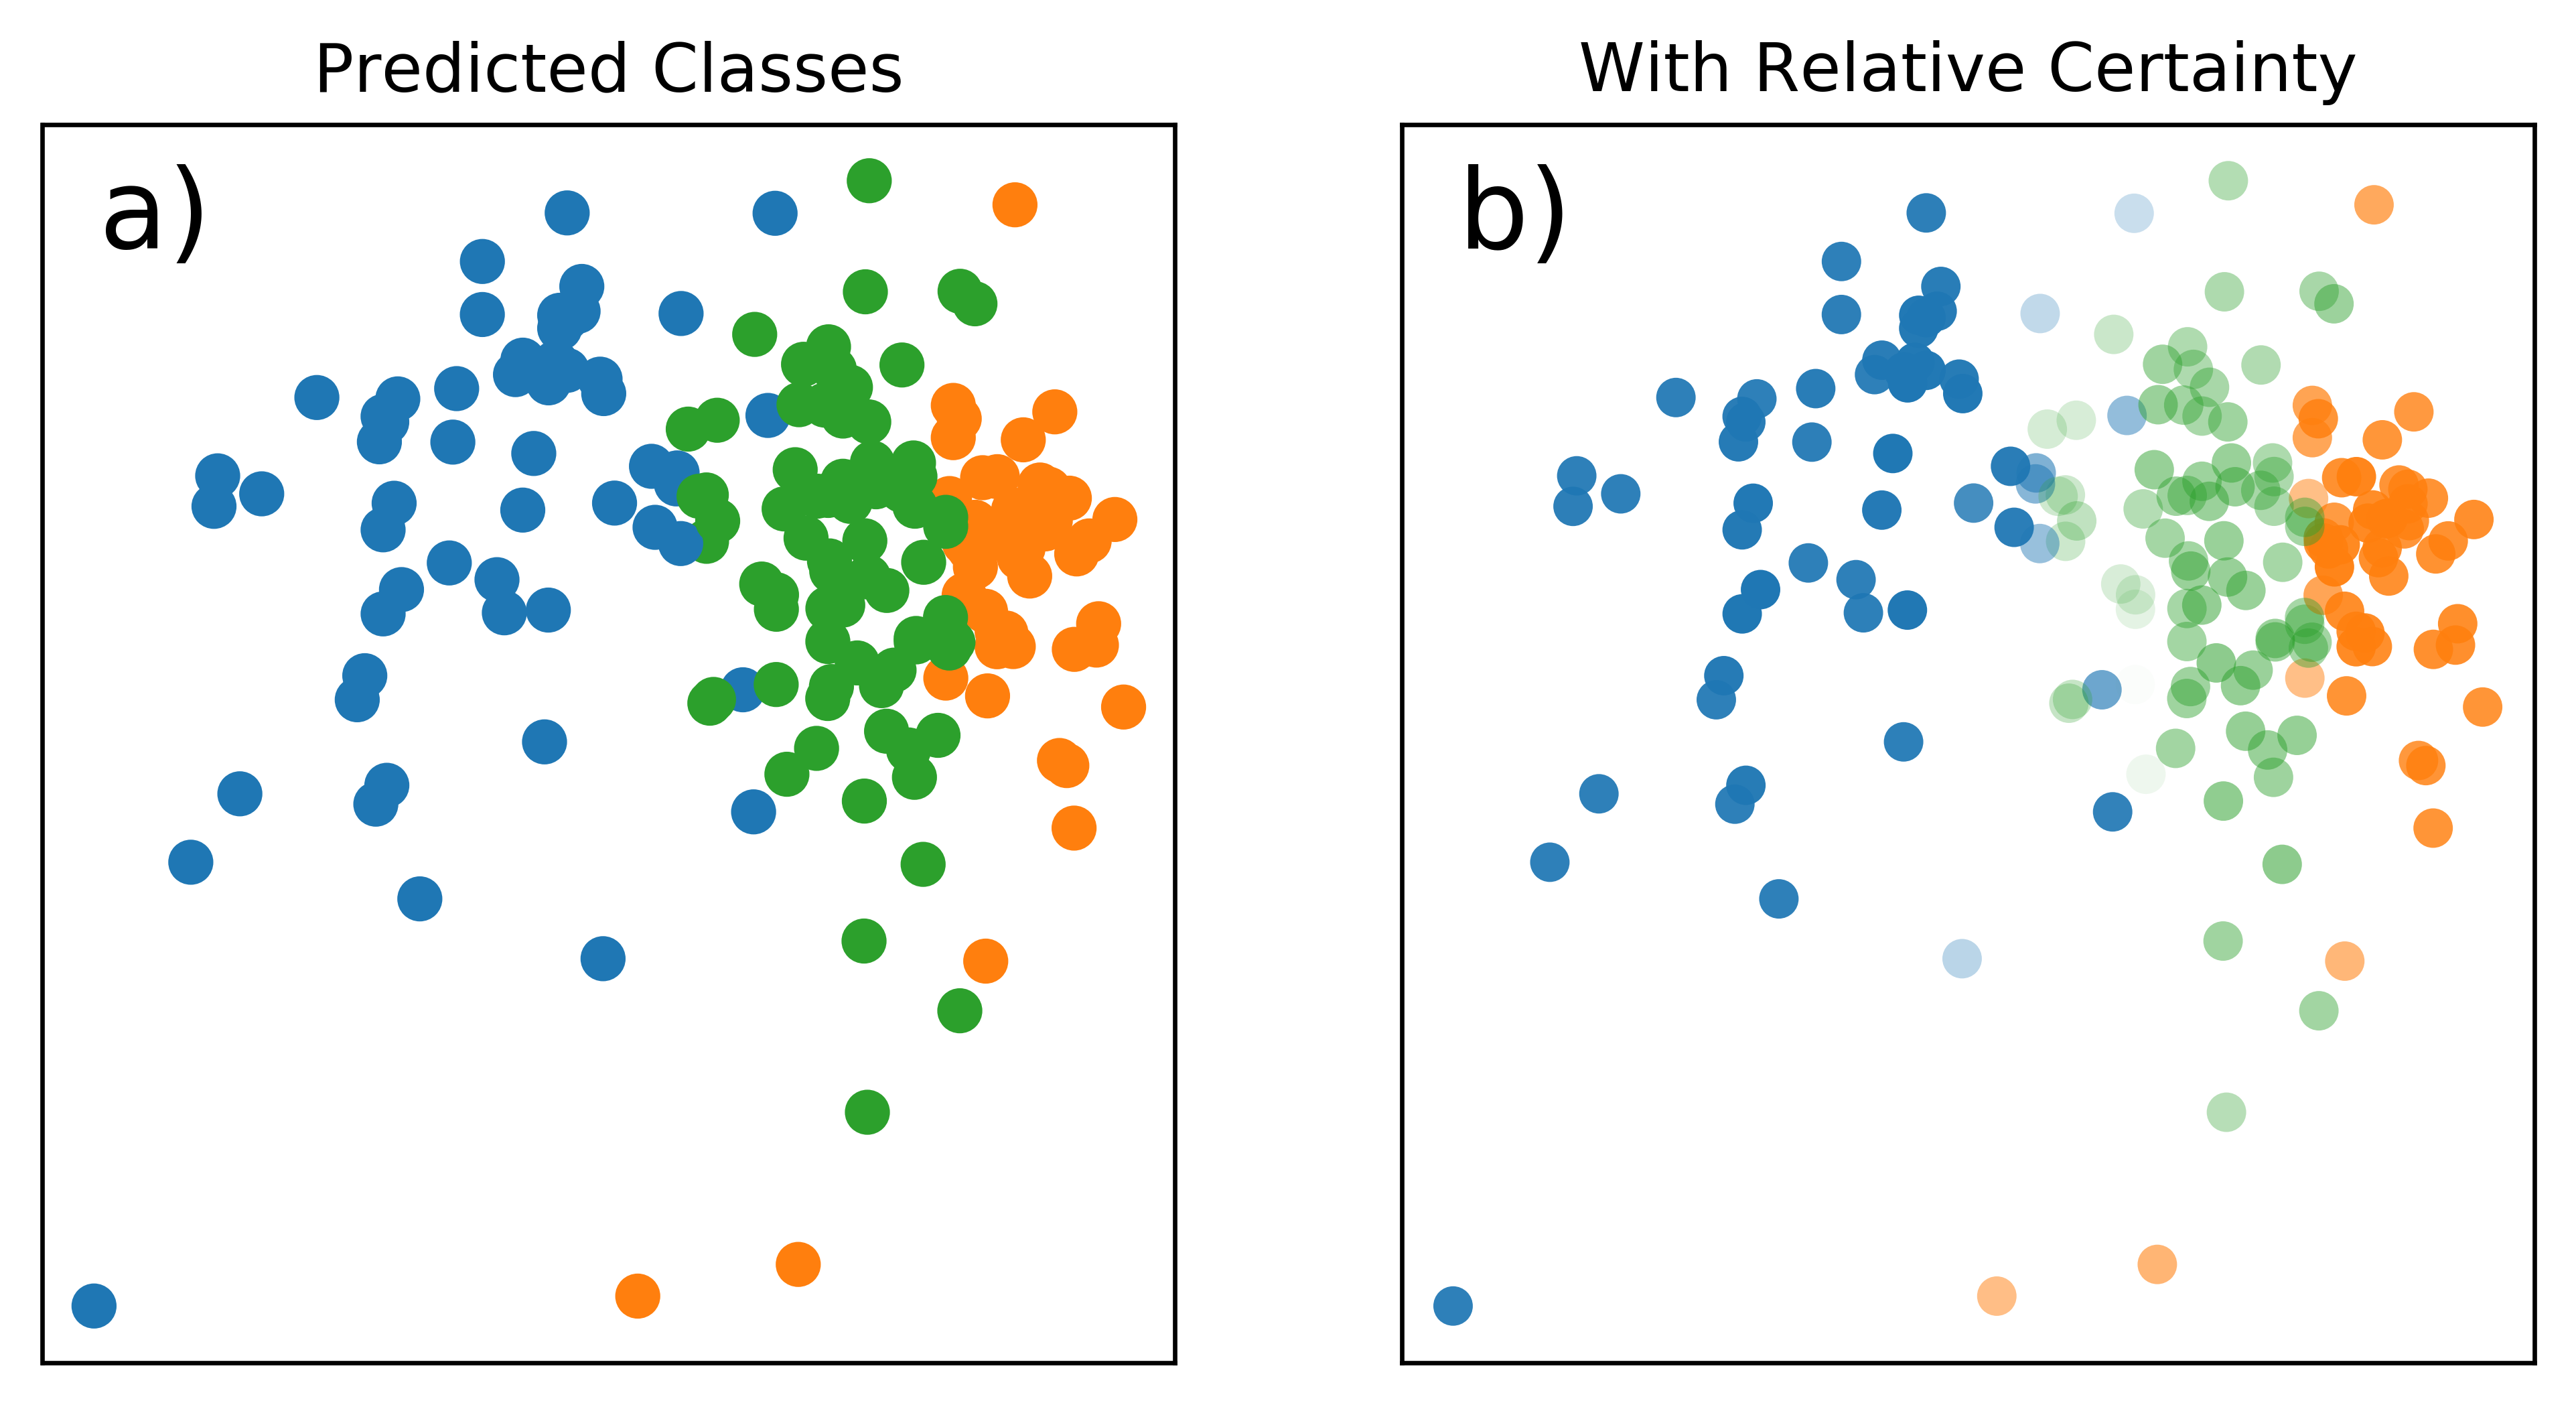
\includegraphics[width=0.8\textwidth]{./figures/manifold_uncertainty_noticks.png}
		\caption[]{Simple example of a visualising spatial relationships and classification uncertainty using a 2D manifold approximation of a small dataset with 13 features, and varying opacity based on a probability entropy measure.  a) Individual analyses coloured by predicted classes; b) analyses coloured by predicted class and relative certainty, highlighting uncertainty away from class centres.}
	\end{figure*}
	
	The analysis approaches documented here contrast with typical geochemical and petrological methods in the level of granularity: here we largely consider analyses individually, while classically analyses are investigated as members of a group or series wherever possible. Differences in trends in geochemistry are arguably more important than absolute differences in geochemical composition, and this information is what is required to differentiate processes. Further work is needed to establish metrics which better represent and contrast geological phenomena, including integrating more diverse information (e.g. context derived from stratigraphic, mineralogical information).
	
	This study focuses on the use of supervised learning, but the use unsupervised learning methods will provide a unique opportunity to assess the significance and validity of human-centric geochemical divisions. This approach may also reveal the presence or absence of physiochemical divides (as one may expect through differences in fractionation etc.). Additionally, with the growing volume of data, more complex probabilistic models may exhibit enhanced performance relative to the simple-but-intuitive support vector classifiers discussed here. 
	
	\subsection*{Conclusions}
	
	Large geochemical databases provide solid foundations for constructing practical machine tectonic discrimination models, which can be adapted for applications from local to global scales. Free and open source tools for constructing classification workflows are readily available. Classification uncertainty across classes and throughout geochemical space can be effectively visualised, and can provide useful insight into the problem at hand. There are practical limits to machine classification of geochemical data, particularly with regard to tectonic discrimination. Some of these lie in the nature of compositional data, others in geological factors (such as preservation biases), and others are issues relating to the representation of data (e.g as individual analyses, rather than linked series of analyses). Major opportunities exist to use more diverse datasets and incorporate semantic knowledge, leveraging the context of samples and their chemistry to hone classification models.
	
	\begin{singlespace*}
	\subsection*{References}
	\footnotesize{
		\bibliography{../../../References/Zotero/ZoteroDB.bib}
	}
	\end{singlespace*}
	\end{multicols*}
	
	
\end{document}